\documentclass[conference]{IEEEtran}
% Include all packages from file.
% Report template for Mälardalen University
% Original template can be found: 
% https://www.overleaf.com/latex/templates/ieee-bare-demo-template-for-conferences/ypypvwjmvtdf
% Template file structure organised by: Emil Persson
% The following packages should follow the IEEE conference guidelines.

% Swedish language package 
\usepackage[utf8]{inputenc}
\usepackage[T1]{fontenc}
\usepackage[english]{babel}

% Graphics
\usepackage{graphicx, float, subfigure, blindtext}
\usepackage{tikz}
\usetikzlibrary{shapes.geometric, arrows, positioning, calc}
\tikzstyle{startstop} = [rectangle, rounded corners, minimum width=1cm, minimum height=0.5cm,text centered, draw=black, fill=red!30,node font=\scriptsize]
\tikzstyle{io} = [trapezium, trapezium left angle=70, trapezium right angle=110, minimum width=1cm, text width=20mm, minimum height=0.5cm, text centered, draw=black, fill=blue!30,node font=\scriptsize]
\tikzstyle{process} = [rectangle, minimum width=1cm, minimum height=0.5cm, text centered,text width=1.2cm, draw=black, fill=orange!30,node font=\scriptsize]
\tikzstyle{decision} = [diamond, minimum width=0.5cm, minimum height=0.5cm, text centered,text width=1.1cm, draw=black, fill=green!30,node font=\scriptsize]
\tikzstyle{arrow} = [thick,->,>=stealth]


\newcommand\IEEEhyperrefsetup{
bookmarks=true,bookmarksnumbered=true,%
colorlinks=true,linkcolor={black},citecolor={black},urlcolor={black}%
}

% Preferred hyperref setup, Michael Shell
\usepackage[\IEEEhyperrefsetup, pdftex]{hyperref}

% Maths
\usepackage{mathtools}

% These packages must be at the end
\usepackage[nolist,nohyperlinks]{acronym}
\usepackage{cleveref}
\graphicspath{{images/}}

% Remove section first paragraph indent
\usepackage{titlesec}
\titlespacing*{\section}{0pt}{*1}{*1}
\titlespacing*{\subsection}{0pt}{*1}{*1}
\renewcommand{\thesubsubsection}{\arabic{subsubsection}}
\titleformat{\subsubsection}[runin]{\itshape}{\thesubsubsection)}{1em}{}[:]
\titlespacing*{\subsubsection}{\parindent}{0pt}{*1}

% Include authors 
\author{\IEEEauthorblockN{ %
Joel Näktergal\IEEEauthorrefmark{1},
Taika Tervola\IEEEauthorrefmark{2}, 
}
\IEEEauthorblockA{
School of Innovation, Design and, Engineering\\
Mälardalens University, Västerås, Sweden\\
Email:
\IEEEauthorrefmark{1}jbl23002@student.mdu.se, 
\IEEEauthorrefmark{2}tta23002@student.mdu.se
}}

% ACRONYMS: \acrodef{acronym}[short name]{full name}
\acrodef{svm}[SVM]{Support Vector Machine}

% The report title.
\title{Game Documentation}
% Document begins here
\begin{document}
% Create the title.
\maketitle
% Example sections, name them
% according to specific needs.
%**********************start*{How to play}*section**********************%
\section{How to play}%
\label{sec:how_to_play}

%**********************start*{Controls}*subsection**********************%
\subsection{Controls}%
\label{sub:controls}
\begin{itemize}
    \item p ; "pauses the game"
    \item i ; "moves the player position one step upwards"
    \item k ; "moves the player position one step downwards"
    \item j ; "moves the player position one step to the left"
    \item l ; "moves the player position one step to the right"
\end{itemize}
%------------------------end-{Controls}-subsection-----------------------%

%**********************start*{Goal of the game}*subsection**********************%
\subsection{Goal of the game}%
\label{sub:goal_of_the_game}
\begin{enumerate}
    \item To hunt the other "*" before it moves.
        \begin{enumerate}
            \item If you make it to its position before it moves, you get a point. The position of the score then changes.
            \item If you are unable to do not make it to the its position before the time runs out, then it will move and the number of tries will be reduced by one.
            \item Once you have missed to catch it 10 times; the game will end.
        \end{enumerate}
\end{enumerate}
%------------------------end-{Goal of the game}-subsection-----------------------%
%**********************start*{System overview}*subsection**********************%
\subsection{System overview}%
\label{sub:system_overview}
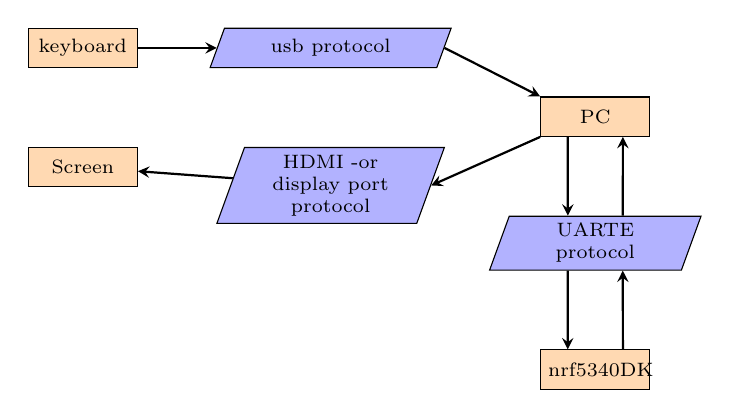
\begin{tikzpicture}[]
    \node[process] (keyboard) {keyboard};
    \node[io,right=of keyboard] (usbprotocol) {usb protocol};
    \node[io,below=of usbprotocol] (hdmiprotocol) {HDMI -or display port protocol};
    \node[process,below=of keyboard] (screen) {Screen};
    \node[process,xshift=20mm] (pc) at ($(usbprotocol.east)!0.5!(hdmiprotocol.east)$) {PC};
    \node[io,below=of pc] (uarte) {UARTE protocol};
    \node[process,below=of uarte] (nrf5340dk) {nrf5340DK};

    \draw[arrow] (keyboard) -- (usbprotocol.west);
    \draw[arrow] (usbprotocol.east) -- (pc.north west);
    \draw[arrow] (pc.south west) -- (hdmiprotocol.east) ;
    \draw[arrow] (hdmiprotocol) -- (screen);
    \draw[arrow] ($(pc.south west)!0.5!(pc.south)$) -- (uarte.north west) ;
    \draw[arrow] (uarte.north east) -- ($(pc.south east)!0.5!(pc.south)$);
    \draw[arrow] (uarte.south west) -- ($(nrf5340dk.north west)!0.5!(nrf5340dk.north)$);
    \draw[arrow] ($(nrf5340dk.north east)!0.5!(nrf5340dk.north)$) -- (uarte.south east);
\end{tikzpicture}
%------------------------end-{System overview}-subsection-----------------------%
%------------------------end-{How to play}-section-----------------------%

% Select the IEEEtran style
\bibliographystyle{IEEEtran}
% Include bibliography file
% \bibliography{IEEEabrv,refs}
\end{document}
